%!TEX root = ..\..\main.tex

\section{Materialien}\label{sec:Materials}
\todo[inline, color=red]{XXX}

\subsection{Hardware}\label{sec:Hardware}
\subsection{Software}

\subsubsection{Klassen}
\todo[inline, color=red]{Artjom}

Im folgenden werden die Methoden der einzelnen Klassen erläutert. Die vollständige UML zur besseren Verständlichkeit der Klassenbeziehungen ist der Abb. \ref{img:UML} zu entnehmen.

\paragraph{point\_grid\_radial\_affin\_distor\_}
Hauptklasse der Anwendung. Implementiert das Interface \emph{PluginFilter} um über ImageJ aufgerufen werden zu können.

Die Klasse besitzt folgende Methoden und deren Funktion:

\begin{table}[H]
\begin{tabular}{p{0.3\textwidth} | p{0.7\textwidth}} 
run & Main-Methode des PlugIns in der die Optimierung aufgerufen wird\\ \hline
setup & Konstruktor-Methode des PlugIns in dem die Bildreferenz gespeichert wird\\ \hline
readData & Liest aus einer in ImageJ geöffneten Textdatei Punkt-Paare ein für Start- und Ziel-Koordinten\\
computeDrawRadialTransformation & \\ \hline
drawTargets & Zeichnet Punkte an den übergebenen Ziel-Koordinaten in das übergebene Bild\\ \hline
computeDrawAffineTransformation & \\ \hline
computeRadius2Center & Berechnet anhand der Parameter den Abstand zum Gittermittelpunkt\\ \hline
compute\_radial\_dist\_koeff & Berechnet mit dem LevenbergMarquadt Optimierer die Koeffizienten der Radialen Verzerrung der übergebenen Punkt und gibt die Koeffizienten zurück\\ 
\end{tabular}
\caption{Methoden der point\_grid\_radial\_affin\_distor\_ Klasse}
\end{table}
\paragraph{SimplePair}
Eine Einfache Klasse zum Speichern der Vorgabe- und Ziel Koordinaten und des Abstandes zum Mittelpunkt.

\paragraph{RadialDistFunction}
Klasse zum Erzeugen der Funktionen für den Optimierer.

\begin{table}[H]
\begin{tabular}{p{0.3\textwidth} | p{0.7\textwidth}} 
RadialDistFunction & Konstruktor der Klasse. Es wird ein SimplePoint Array erwartet welcher Koordinaten-Paare für Start- und Ziel-Koordinaten enthält.\\ \hline
realTargetPoints & Gibt ein Array aus welches nur die Ziel-Koordinaten enthält. Dieses wird für den Optimierer benötigt.\\ \hline
retMVF & Funktion zur Modellierung der Radialen Verzerrung für den Optimierer. BErechnet zu den Vorgegeben Koeffizienten und einer Start-Koordinate die Ziel-Koordinate\\ \hline
retMMF & Jacobi-Matrix-Funktion zur Berechnung der Ableitung nach den einzelnen vom Optimierer vorgegebenen Koeffizienten \\ 
\end{tabular}
\caption{Methoden der RadialDistFunction Klasse}
\end{table}

\begin{figure}[H]
\center
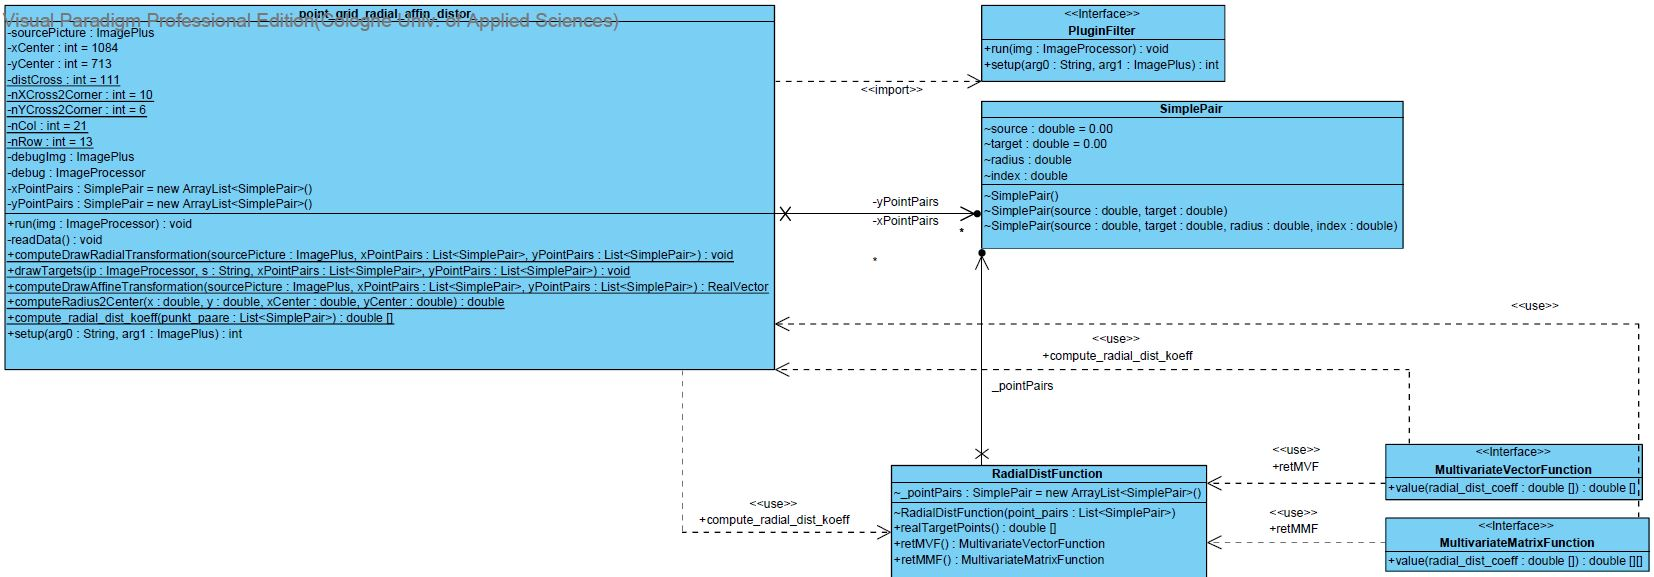
\includegraphics[width=\textwidth]{Images/UML.JPG}
\caption{UML Klassendiagramm}
\label{img:UML}
\end{figure}



\subsubsection{ImageJ}
\newpage
